\chapter{基于SDN的云平台架构设计}
基于SDN的云平台多租户虚拟网络定制化的研究,主要是将SDN集中控制和可编程的优势,集成到云数据中心,通过网络虚拟化技术,为租户提供相互隔离的vSDN网络,vSDN网络由租户自由的控制器实现集中管控。物理网络的集中管控,方便运营商对数据中心网络的管理和维护;租户vSDN网络的集中控制,便于租户利用自己的控制期开发适合自己的上层应用。本章最该研究的主要架构进行简单的介绍。
\section{关键技术分析}
\subsection{需求分析}
基于SDN的云平台多租户虚拟网定制化的实现,首先解决的是物理网络资源的虚拟化,其次是在虚拟化的基础上进行虚拟网络的带宽时延测量,随后根据测量的带宽时延进行链路的定制化,最后为方便用户的操作,完成前端Web界面的设计和实现。

系统的整体需求如图\ref{fig:ovx}所示。

\begin{figure}[!htb]
  \centering
  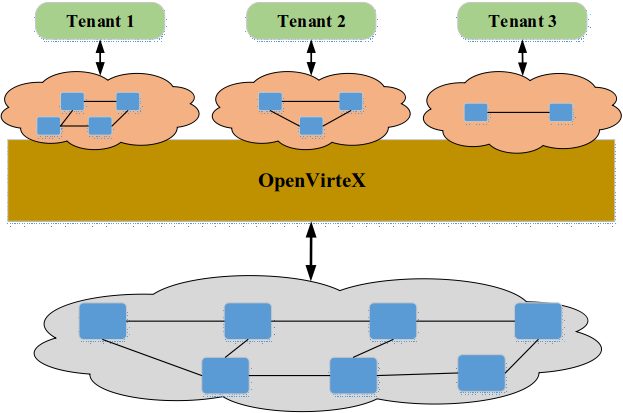
\includegraphics[width=0.7\textwidth]{logo/ovx.png}
  \caption{OVX网络虚拟化示意图}
  \label{fig:ovx}
\end{figure}

网络的虚拟化,需要实现资源隔离的同时,还要满足虚拟网络支持SDN模式,本文选用支持资源虚拟化的SDN控制器来完成该功能,通过对底层物理网络中下发的流表信息中,添加租户ID的相关信息,完成底层网络中租户的隔离工作。通过自身维护的物理网络与虚拟网络的映射关系图,为上层SDN交换机提供支持OpenFlow协议的虚拟网络,此时租户便可利用自身的SDN控制器完成对vSDN网络的集中管控。

在虚拟资源之上进行链路带宽时延等信息的测量工作,需要实现SDN模式下链路的带宽、时延的精确测量,由于SDN的集中控制和可编程的先天优势,控制器端可以看到全局的网络拓扑,与此同时,OpenFlow协议的规范性和便捷性,方便了我们实现可用带宽、已用带宽、时延的精确测量工作,测量的数据成为用户做出决策的考量值。

链路的定制化,需要用户根据链路的时延、带宽等信息,选取便于传输的最优链路,进行定制化流表的下发工作,此时,租户便可以对自己在数据中心的虚拟机,进行远程的操控,可以自定义数据的传输路径。

前端的Web界面方便了用户的操作,用户可以在其web界面,通过简单的点击操作,完成对数据中心网络的定制化操作。包括物理、虚拟网络的拓扑获取,链路带宽、时延的前端展示,虚拟网络的创建,定制化链路的前端选取等功能。一系列的操作,需要实现租户之间的隔离工作,我们需要通过认证功能,对租户的请求进行认证。实现租户操作的隔离行。

\subsection{关键技术}

\section{系统架构设计}
\subsection{系统总体设计图}
系统主要由四个模块组成。分别为网络虚拟化模块、控制器模块、通信模块和GUI模块。总体的架构图如图\ref{fig:ovx}所示。

\begin{figure}[!htb]
  \centering
  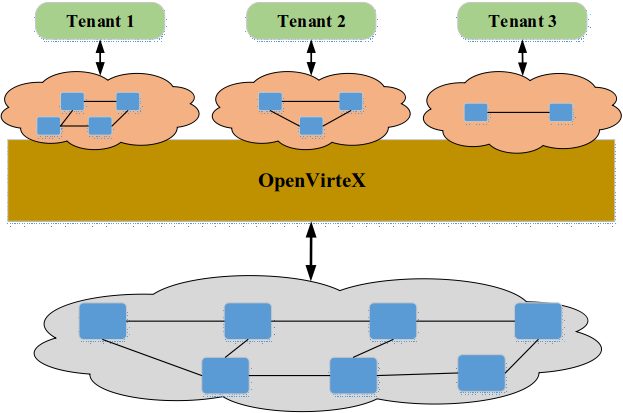
\includegraphics[width=0.7\textwidth]{logo/ovx.png}
  \caption{OVX网络虚拟化示意图}
  \label{fig:ovx}
\end{figure}

如图中所示,架构底层主要包含支持OpenFlow协议的交换机,以及OpenStack内部的虚拟机资源,交换机既包含OpenStack内部的虚拟网桥,亦包含连接物理服务器之间的物理OpenFlow交换机。将这部分网络开放给租户,主要是为了便于租户实现对数据中心物理网络的可控性。租户可以根据链路时延、带宽定制化最优数据传输链路。支持网络虚拟化的SDN控制器,实现对底层网络和计算资源的集中控制。由该模块,可以创建相互隔离的租户虚拟网络,该虚拟网络支持SDN模式,租户可利用控制器实现对自由虚拟网络的集中管控。自主开发北向应用,实现特有的功能。

控制器模块主要实现对租户控制器的管理。租户的控制器实现对自有vSDN网络的集中管控,该控制器运行于特定虚拟机之中,租户可以登录虚拟机,进行相应的配置和开发工作。每一个vSDN网络对应唯一的SDN控制器。现有的控制器镜像,已经开发了对链路带宽、时延的测量功能,租户可以登录控制器所在的虚拟机,开发自己的北向应用。

通信模块主要实现异步通信,前端对网络拓扑的获取、带宽时延数据的获取以及虚拟网络的创建请求,均通过通信模块,分别和控制器、网络虚拟化模块完成数据的请求和获取。通信模块完成了进程间的异步通信。

前端GUI界面,主要为了方便用户的操作,用户可以在其web界面,通过简单的点击操作,完成对数据中心网络的定制化操作。包括网络拓扑的显示,链路带宽、时延的前端展示,虚拟网络的创建操作,定制化链路的前端选取等功能。前端模块的极大的提高了用户体验效果。

\subsection{系统详细架构图}
在OpenStack云平台数据中心网络中采用SDN架构,核心思想是用控制器对网路运营模式实现统一管控。现有云数据中心网络的模式均为单一节点控制,该模式下的SDN网络对于租户是不可见的。本文提出了多租户虚拟化网络的定制和管理方案,实现了租户自有控制器对虚拟网络的灵活控制。多租户对应多控制器的机制便于租户对自有网络进行带宽时延查询、定制化流表下发、链路切换、控制器北向接口开发实验等自定义操作。系统的详细架构图如图\ref{fig:architecture}所示。

\begin{figure}[!htb]
  \centering
  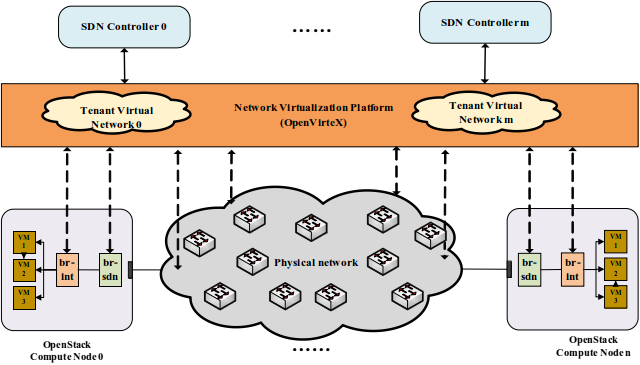
\includegraphics[width=0.7\textwidth]{logo/architecture.png}
  \caption{系统详细架构图}
  \label{fig:architecture}
\end{figure}

在兼容现有OpenStack网络模式的前提下,为OpenStack平台的每个计算节点添加br-sdn网桥,用于完成SDN网络模式下的数据转发。架构主要由四个模块组成,分别为云数据中心网络边缘侧的OpenStack云平台、云数据中心侧物理网络与虚拟网络映射模块、SDN控制器模块、通信模块。对于OpenStack云平台,本文选取Kilo版本进行搭建;云数据中心物理网络与虚拟网络的映射模块由OpenVirtex(简称OVX,开源网络虚拟化工具)实现[10],对开源软件OVX内部的映射算法进行了更新,基于粒子群算法实现该映射模块,提高了物理资源的利用率;控制器模块实现对租户vSDN网络的集中管控,控制器与vSDN网络之间一一对应,租户自定义控制器,实现对自有vSDN网络的集中控制,便于租户对网络管控的同时,可以根据控制器的反馈查询网络异常原因,同时亦可开发北向应用,实现对网络的灵活管控;通信模块主要实现OpenStack网络组件Neutron[11]与OVX之间的通信,本文基于RabbitMQ[12]实现,完成了Neutron侧指令的下发、OVX侧测量结果的返回。
\subsection{系统流程图}
系统的整体流程图如图\ref{fig:workflow}所示。

\begin{figure}[!htb]
  \centering
  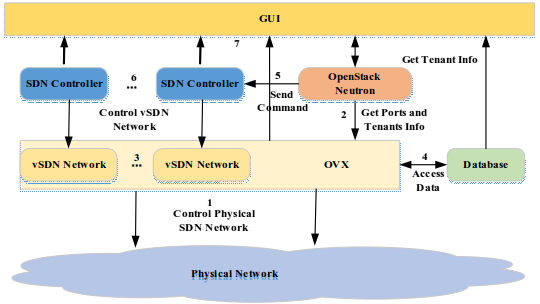
\includegraphics[width=0.7\textwidth]{logo/workflow.png}
  \caption{系统详细流程图}
  \label{fig:workflow}
\end{figure}

\begin{enumerate}
\item OVX实现对底层物理网络管理,完成物理网络的集中控制,本文为其开发了创建虚拟网络的API接口createCustomNetwork以及基于粒子群的虚拟网络映射模块。
\item 调用OpenStack Neutron的API接口,获取虚拟机的端口信息,与OVX本身获取的交换机信息组合,得到整个物理网络的拓扑信息。
\item 调用OVX的createCustomNetwork接口,完成虚拟网络的创建。
\item 每一个虚拟网络由ID号virtualnetworkid进行标识。在OpenStack中,每个租户有自己的ID号tenantid。本文将两者的对应关系存储到数据库中。
\item OpenStack Neutron侧通过RabbitMQ发送指令到SDN控制器。现阶段,指令主要包括带宽/延迟测量以及定制化流表的下发。未来我们的平台将提供更多的功能。
\item SDN控制器接收到消息,通过我们开发的应用,完成相应的测量工作。最后返回对应的数据。租户可以开发自己的应用程序,以实现更多的功能。
\item GUI界面完成物理网络、虚拟网络、链路带宽、时延等信息的获取,在前端界面实现展示工作。
\end{enumerate}

\section{模块详解}
\subsection{网络虚拟化模块}

虚拟化的计算资源和存储资源最终都需要通过网络为用户提
供访问。如何让云中各种类型的用户尽可能安全的使
用网络,如何让用户无缝的接入和使用云计算服务,
以及通过网络满足数据中心间的数据传输和迁移,标
准组织和设备厂商都在积极的研究,并提出了解决方
案。其中通过虚拟化技术提高网络的利用率,并让网
络具有灵活的可扩展性和可管理性,是云计算网络研
究的热点。在网络领域中,虚拟化并不是一项新兴技
术,虚拟网络允许不同需求的用户组访问同一个物理
网络,但从逻辑上对它们进行一定程度的隔离,以确
保安全。凭借网络虚拟化技术,能在单一物理基础设
施上部署多个封闭用户组,并在整个网络中保持高标
准的安全性、可扩展性、可管理性和可用性。通过网
络虚拟化可实现弹性、安全、自适应、易管理的基础
网络,充分满足服务器虚拟化等虚拟技术对基础网络
带来的挑战,达到提高数据中心的运行效率、业务部
署灵活、降低能耗、释放机架空间的目的。

网络虚拟化允许多个租户占据相同的网络基础设施,每个租户会有一种错觉,认为可以对整个网络进行完整的处理,对于网络映射模块,本文选用OVX,OVX通过给每个租户提供访问一个虚拟网络拓扑和一个完整的网络头空间来达到这样的目标,前者允许租户自定义拓扑结构,而后者保证功能性和流量隔离,即使是在不同的租户选择重叠的寻址方案。OVX用作控制信道内的一个代理,呈现OpenFlow网络给租户,同时经由南向的OpenFlow接口控制底层的物理基础设施。图2描述了此结构。通过暴露OpenFlow网络给租户,OVX允许租户使用自己的网络控制器控制自有的虚拟网络资源。换句话说,OVX基于同一底层物理网络创建多个SDN虚拟网络,并且SDN虚拟网络之间是相互隔离的,保证了租户虚拟网络的安全性。这样的方法会产生两个后果:,允许OVX呈现支持OpenFlow的可编程虚拟网络,租户可以使用自己的NOS控制虚拟网络,使OVX是透明的——从底层网络的角度,OVX的表现为一个控制器,从租户的角度上看,OVX作为网络中具有OpenFlow能力的交换机集合。

\begin{figure}[!htb]
  \centering
  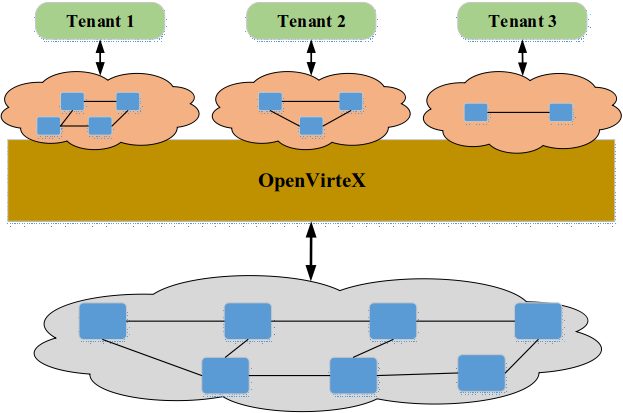
\includegraphics[width=0.7\textwidth]{logo/ovx.png}
  \caption{OVX网络虚拟化示意图}
  \label{fig:ovx}
\end{figure}

\subsection{通信模块}
通信模块基于RabbitMQ实现,消息队列是一种应用程序对应用程序的通信方法。应用程序通过读写出入队列的消息(针对应用程序的数据)来通信,而无需专用连接来链接它们。消息传递指的是程序之间通过在消息中发送数据进行通信,而不是通过直接调用彼此来通信。RabbitMQ作为消息代理,给应用程序提供一个共同的平台,用于存储发送/接受的消息。知道消息从队列中被接收端收到为止。

\subsection{控制器模块}
本文选用Ryu控制器,Ryu是一个基于组件的软件定义网络架构,是一个基于Apache协议的完全开源的SDN控制器,对于软件组件提供了良好的API接口,便于开发人员创建新的网络管理与控制中的应用,Ryu支持管理网络设备的多种网络协议,诸如:OpenFlow,Netconf,OF-config等,本文在Ubuntu镜像中集成该控制器,租户根据自身需求,利用该镜像创建合适大小的虚拟机,从而实现对自有虚拟SDN网络的集中控制,租户可以根据自身需求进行控制器北向应用的相关开发工作。本文主要实现了链路的时延、带宽的测量,以及定制化流表的下发实验。

Ryu是一个基于组件的软件定义网络架构。刘某提供的软件组件具有定义良好的API,便于开发人员创建新的网络管理与控制中的应用。刘某支持管理网络设备的各种协议,如OpenFlow,NETCONF,配置,等所有的代码都是免费提供的Apache 2许可证。

\subsection{GUI模块}
基于OpenStack的Horizon模块,集成相关的前端操作,显示云数据中心物理拓扑,以及链路的带宽、时延,租户根据物理网络的相关参数创建自有的SDN虚拟网络,并指定某一控制器对该虚拟网络实现集中管控。对于租户的虚拟网络,前端界面主要负责显示拓扑信息、链路带宽、时延等信息,租户亦可根据链路状态,进行定制化流表的下发,从而实现链路的切换。所有的这些操作的反馈信息,均在前端展示给租户,租户根据信息的正确与否进行相应的解决方案。
\section{本章小结}